\section{简单样板图样}\label{sec:yangban}
{\bfseries 知识目标}
\begin{itemize}
\item 掌握rectang命令的使用方法
\item 掌握chamfer命令的使用方法
\item 掌握offset命令的使用方法
\item 掌握break命令的使用方法
\item 掌握fillet命令的使用方法
\end{itemize}
{\bfseries 技能目标}
\begin{itemize}
\item 具备绘制中复杂程度的图样的能力
\item 具备图样尺寸分析的能力
\item 具备一定的AutoCAD图形编辑能力
\end{itemize}
\begin{figure}[htbp]
\centering
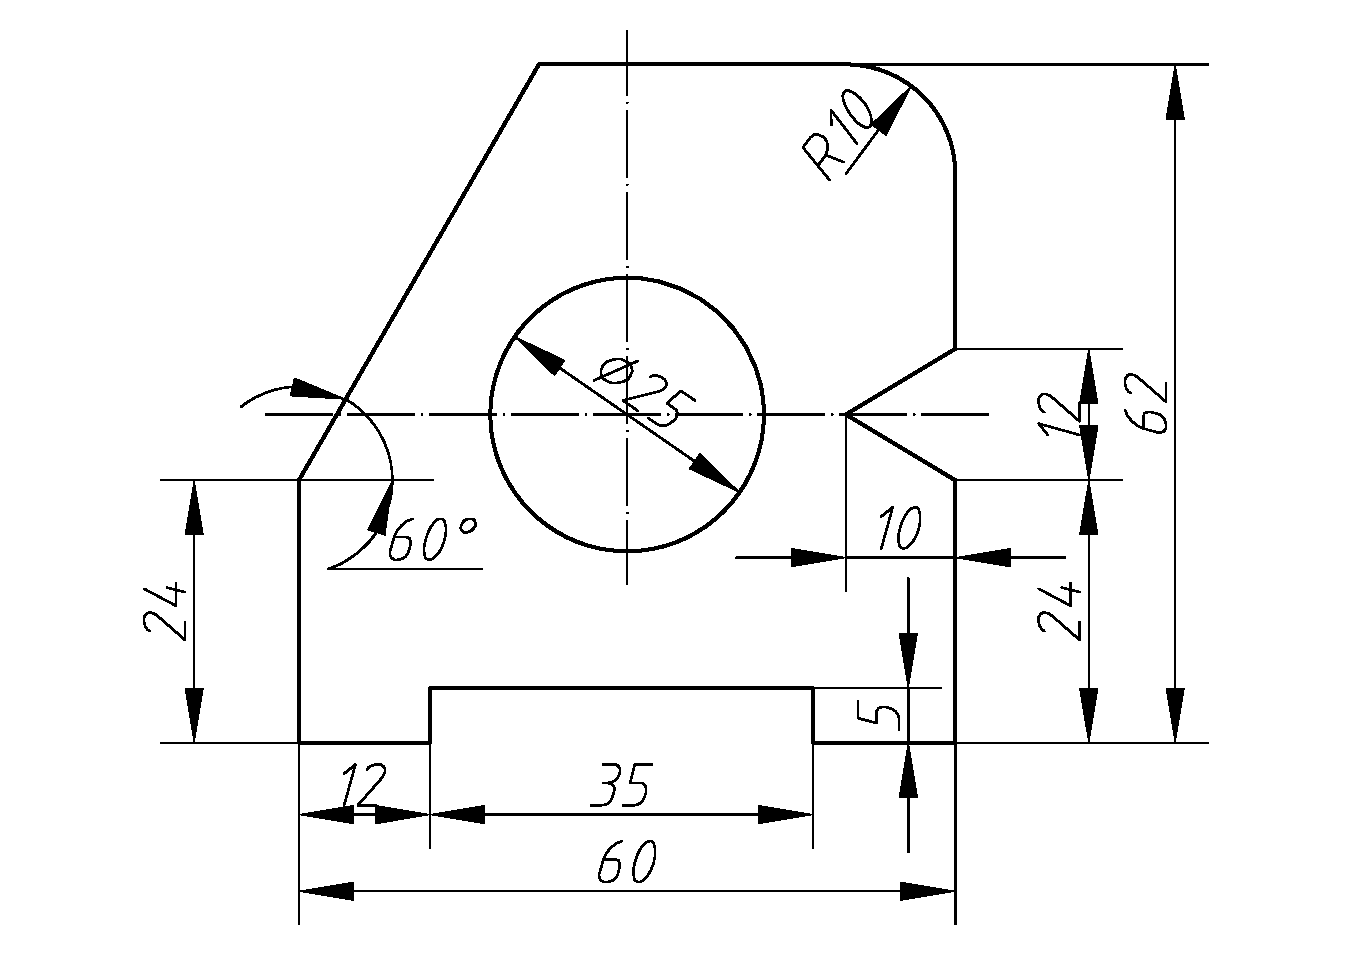
\includegraphics[scale=0.45]{shu4.pdf}
\caption{简单样板图样}\label{fig:renwu3}
\end{figure}
\subsection{绘制图样}
首先,我们来绘制图\ref{fig:renwu3}所示的图样。

第一步:设置图层,具体设置方法参见\ref{sec:falan},此处不再重复。

第二步:绘制中心线,先将中心线图层设置为当前图层。
\noindent
命令: XLINE 指定点或 [水平(H)/垂直(V)/角度(A)/二等分(B)/偏移(O)]: 30,30\\
指定通过点: @1$<$0\\
指定通过点: @1$<$90\\
指定通过点:\\
\indent
第三步:绘制实线,将实线图层设置为当前图层。

\noindent
命令: rectang\\
指定第一个角点或 [倒角(C)/标高(E)/圆角(F)/厚度(T)/宽度(W)]: 0,0\\
指定另一个角点或 [面积(A)/尺寸(D)/旋转(R)]: 60,62\\
命令:offset\\
当前设置: 删除源=否  图层=源  OFFSETGAPTYPE=0\\
指定偏移距离或 [通过(T)/删除(E)/图层(L)] $<1.0000>$:  3\\
选择要偏移的对象,或 [退出(E)/放弃(U)] $<$退出$>$:\\
指定要偏移的那一侧上的点,或 [退出(E)/多个(M)/放弃(U)] $<$退出$>$:\\
选择要偏移的对象,或 [退出(E)/放弃(U)]$<$退出$>$:\\
命令: trim\\
当前设置:投影=UCS,边=无\\
选择剪切边...\\
选择对象或 $<$全部选择$>$:  找到 1 个\\
选择对象:\\
选择要修剪的对象,或按住 Shift 键选择要延伸的对象,或
[栏选(F)/窗交(C)/投影(P)/边(E)/删除(R)/放弃(U)]:\\
选择要修剪的对象,或按住 Shift 键选择要延伸的对象,或
[栏选(F)/窗交(C)/投影(P)/边(E)/删除(R)/放弃(U)]:\\
选择要修剪的对象,或按住 Shift 键选择要延伸的对象,或
[栏选(F)/窗交(C)/投影(P)/边(E)/删除(R)/放弃(U)]:\\
选择要修剪的对象,或按住 Shift 键选择要延伸的对象,或
[栏选(F)/窗交(C)/投影(P)/边(E)/删除(R)/放弃(U)]:\\
选择要修剪的对象,或按住 Shift 键选择要延伸的对象,或
[栏选(F)/窗交(C)/投影(P)/边(E)/删除(R)/放弃(U)]:\\
命令: erase 找到 1 个\\
命令: CIRCLE\\
指定圆的圆心或 [三点(3P)/两点(2P)/切点、切点、半径(T)]: int 于\\
指定圆的半径或 [直径(D)]: 12.5\\
命令:  CHAMFER\\
(“修剪”模式) 当前倒角距离 1 = 0.0000,距离 2 = 0.0000
选择第一条直线或 [放弃(U)/多段线(P)/距离(D)/角度(A)/修剪(T)/方式(E)/多个(M)]:  a \\
指定第一条直线的倒角长度 $<$0.0000$>$: 38 \\
指定第一条直线的倒角角度 $<$0$>$: 30\\
选择第一条直线或 [放弃(U)/多段线(P)/距离(D)/角度(A)/修剪(T)/方式(E)/多个(M)]:\\
选择第二条直线,或按住 Shift 键选择直线以应用角点或 [距离(D)/角度(A)/方法(M)]:\\
命令: fillet\\
当前设置: 模式 = 修剪,半径 = 0.0000\\
选择第一个对象或 [放弃(U)/多段线(P)/半径(R)/修剪(T)/多个(M)]: r \\
指定圆角半径$<$0.0000$>$: 10\\
选择第一个对象或 [放弃(U)/多段线(P)/半径(R)/修剪(T)/多个(M)]:\\
选择第二个对象,或按住 Shift 键选择对象以应用角点或 [半径(R)]:\\
命令: break 选择对象:\\
指定第二个打断点 或 [第一点(F)]: f\\
指定第一个打断点:\\
指定第二个打断点: @0,0\\
命令: chamfer\\
(“修剪”模式) 当前倒角长度 = 24.0000,角度 = 30\\
选择第一条直线或 [放弃(U)/多段线(P)/距离(D)/角度(A)/修剪(T)/方式(E)/多个(M)]:  t\\
输入修剪模式选项 [修剪(T)/不修剪(N)] $<$修剪$>$: n
选择第一条直线或 [放弃(U)/多段线(P)/距离(D)/角度(A)/修剪(T)/方式(E)/多个(M)]:  d 指定 第一个 倒角距离 $<0.0000>$: 6\\
 指定 第二个 倒角距离 $<6.0000>$: 10\\
选择第一条直线或 [放弃(U)/多段线(P)/距离(D)/角度(A)/修剪(T)/方式(E)/多个(M)]:
选择第二条直线,或按住 Shift 键选择直线以应用角点或 [距离(D)/角度(A)/方法(M)]:
命令:CHAMFER
(“不修剪”模式) 当前倒角距离 1 = 6.0000,距离 2 = 10.0000\\
选择第一条直线或 [放弃(U)/多段线(P)/距离(D)/角度(A)/修剪(T)/方式(E)/多个(M)]:  d \\
指定 第一个 倒角距离 $<6.0000>$: \\
指定 第二个 倒角距离$<10.0000>$:\\
选择第一条直线或 [放弃(U)/多段线(P)/距离(D)/角度(A)/修剪(T)/方式(E)/多个(M)]:\\
选择第二条直线,或按住 Shift 键选择直线以应用角点或 [距离(D)/角度(A)/方法(M)]:\\
命令: trim\\
当前设置:投影=UCS,边=无\\
选择剪切边...\\
选择对象或$<$全部选择$>$:  找到 1 个\\
选择对象: 找到 1 个,总计 2 个\\
选择对象:\\
选择要修剪的对象,或按住 Shift 键选择要延伸的对象,或
[栏选(F)/窗交(C)/投影(P)/边(E)/删除(R)/放弃(U)]:\\
选择要修剪的对象,或按住 Shift 键选择要延伸的对象,或
[栏选(F)/窗交(C)/投影(P)/边(E)/删除(R)/放弃(U)]:\\
选择要修剪的对象,或按住 Shift 键选择要延伸的对象,或
[栏选(F)/窗交(C)/投影(P)/边(E)/删除(R)/放弃(U)]:\\
命令: line 指定第一点: 12,0\\
指定下一点或 [放弃(U)]: @5$<$90\\
指定下一点或 [放弃(U)]: @35$<$0\\
指定下一点或 [闭合(C)/放弃(U)]:   @-5$<$90\\
指定下一点或 [闭合(C)/放弃(U)]:\\
命令: trim\\
当前设置:投影=UCS,边=无\\
选择剪切边...\\
选择对象或$ <$全部选择$>$:  找到 1 个\\
选择对象: 找到 1 个,总计 2 个\\
选择对象:\\
选择要修剪的对象,或按住 Shift 键选择要延伸的对象,或
[栏选(F)/窗交(C)/投影(P)/边(E)/删除(R)/放弃(U)]:\\
选择要修剪的对象,或按住 Shift 键选择要延伸的对象,或
[栏选(F)/窗交(C)/投影(P)/边(E)/删除(R)/放弃(U)]:\\
\indent
在完成这个任务的过程中,我们使用到了几个新的命令,现在我们来解释这些命令的相关参数。

 rectang命令用于创建形,其中【倒角(C)】表示指定矩形的倒角距离;【标高(E)】表示指定矩形的标高;【圆角(C)】表示指定矩形的圆角半径;【厚度(F)】表示指定矩形的厚度;【宽度(W)】表示为要绘制的矩形指定多段线的宽度。
 
offset命令用于创建同心圆、平行线和平行曲线,其中【通过(T)】表示创建通过指定点的对象;【删除(E)】表示偏移源对象后将其删除;【图层(L)】表示确定将偏移对象创建在当前图层上还是源对象所在的图层上;【多个(M)】表示使用当前偏移距离重复进行偏移操作;【退出(E)】表示退出offset命令;【放弃(U)】表示恢复前一个偏移。

 CHAMFER命令用于给对象添加倒角,其中【多段线(P)】表示对整个二维多段线倒角;【距离(D)】表示设定倒角至选定边端点的距离;【角度(A)】表示用第一条线的倒角距离和第二条线的角度设定倒角距离;【修剪(T)】表示控制 CHAMFER 是否将选定的边修剪到倒角直线的端点;【方式(E)】表示控制 CHAMFER 使用两个距离还是一个距离和一个角度来创建倒角;【多个(M)】表示为多组对象的边倒角。

fillet命令用于给对象加圆角,其中参数【多段线(p)】、【修剪(T)】和【多个(M)】选项的含意与chamfer命令的含意一致,【半径(R)】用于指定圆角的半径。

break命令用于在两点之间打断选定对象;其中参数【第一点(F)】表示用指定的新点替换原来的第一个打断点。
\zhishi{平面图形分析}
通过\ref{sec:gongzhi}-\ref{sec:yangban}的学习,我们已经学会了一些基本图样的绘制方法和步骤,但是要绘制复杂的图样,则需要了解一定的平面图形分析知识,才能够更准确快捷的绘出图样。图样上的图形是平面图形,需要用尺寸确定组成图样的若干封闭线框的形状(定形尺寸)和相互位置(定位尺寸)。这些形(图形)和数(尺寸)的关系对于设计和加工人员来说是十分重要的。因此,我们必须要弄清楚图形与尺寸之的关系。

\subsection{平面图形的尺寸分析}
尺寸分析包括尺寸基准、定形尺寸和定位尺寸的分析。


\noindent
\begin{figure}[htbp]
\centering
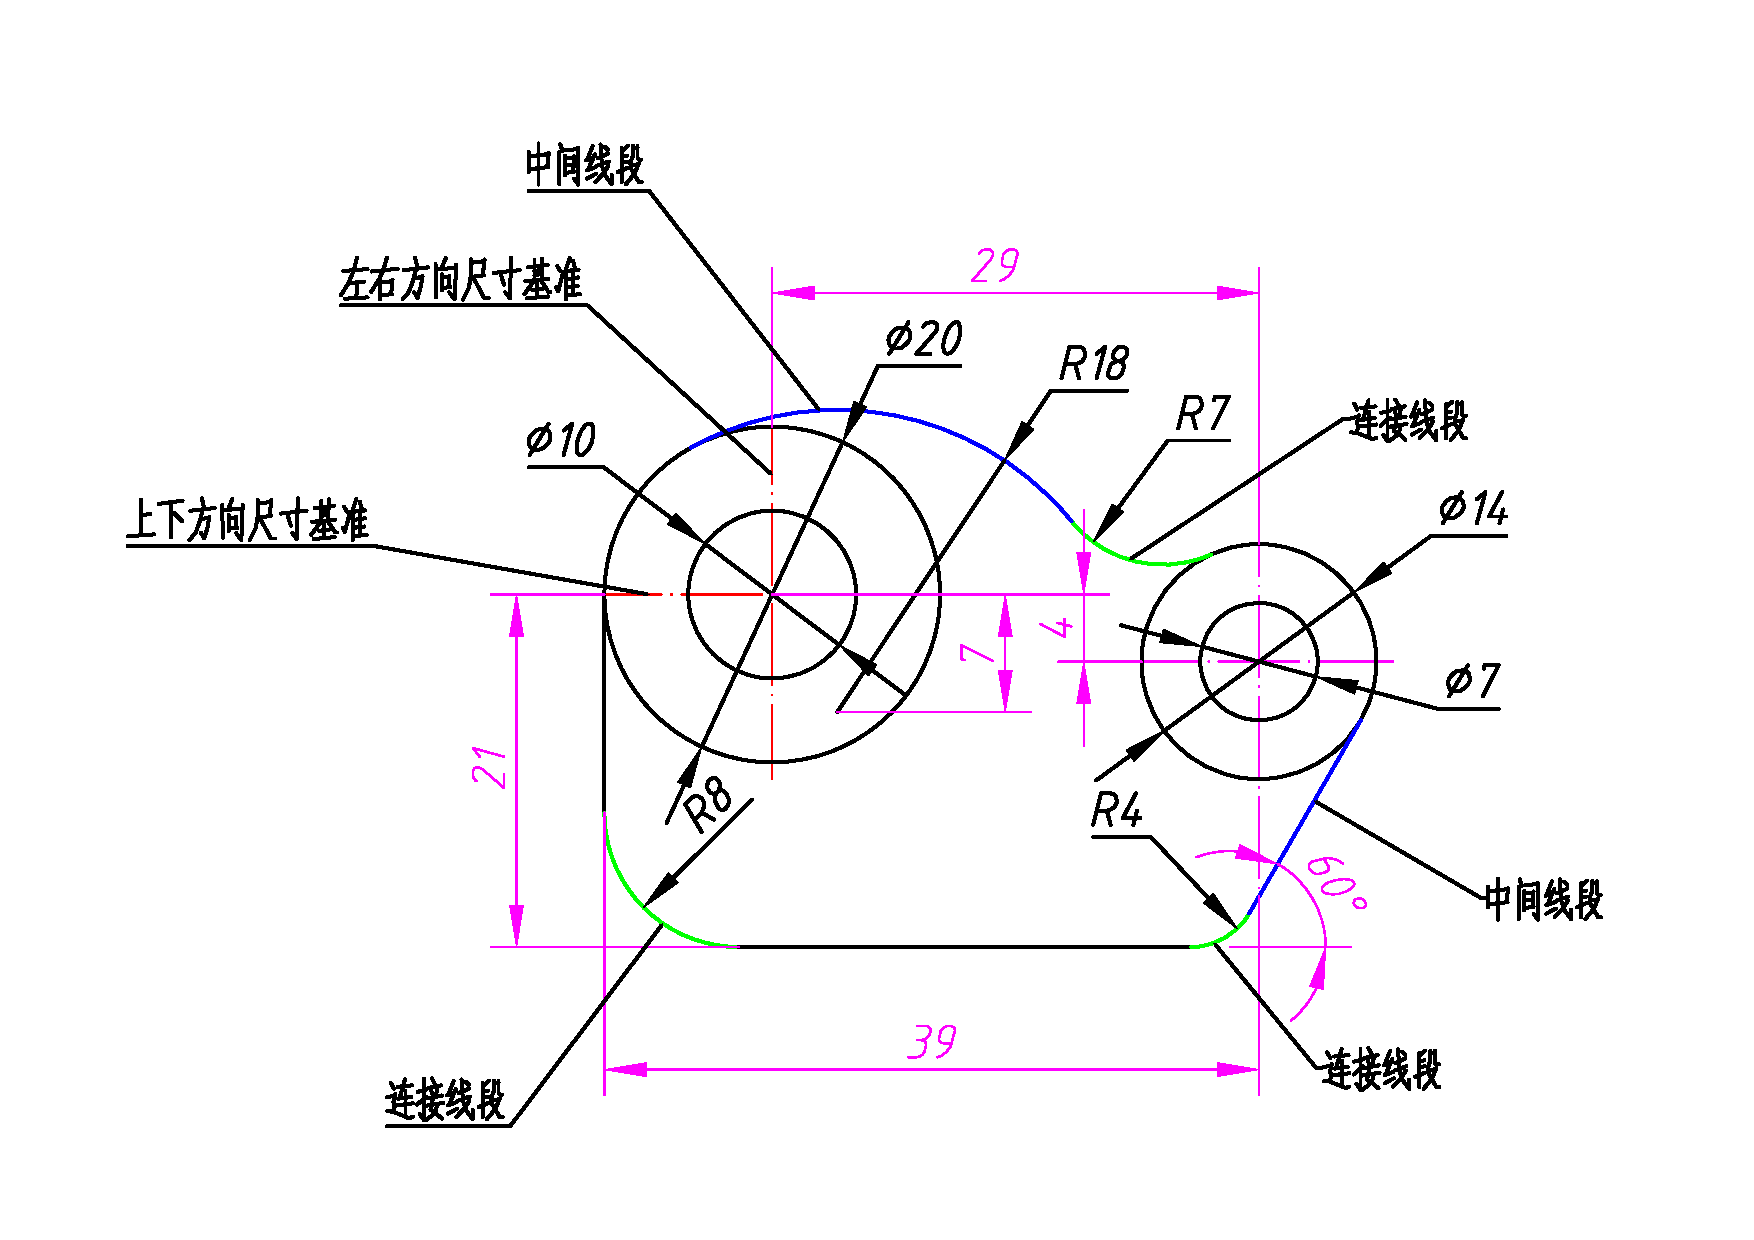
\includegraphics[scale=0.45]{biaozu.pdf}
\caption{平面图形的尺寸和线段分析} \label{fig:biaozu}
\end{figure}
\indent

\begin{enumerate}
\item 尺寸基准

尺寸基准是标注尺寸的起点。一般应有两个方向的尺寸基准。通常情况下,平面图形主要采用图形的对称中心线,较大圆的中心线或主要轮廓线作为尺寸基准线。如图\ref{fig:biaozu}所示,则是采用$\phi 20$圆的中心线作为上下方向和左右方向的尺寸基准。

\item 定形尺寸

定形尺寸是确定平面图形中各线段形状大小的尺寸,如直线的长度、圆和圆弧的直径或半径、角度的大小等。图\ref{fig:biaozu6}所标出的$\phi 10$、$\phi 20$、 $\phi 14$、 $R8$、$R18$、$R7$等尺寸均为图\ref{fig:biaozu}的定形尺寸。

\noindent
\begin{figure}[htbp]
\centering
\begin{floatrow}
\ffigbox{\caption{定形尺寸}\label{fig:biaozu6}}{
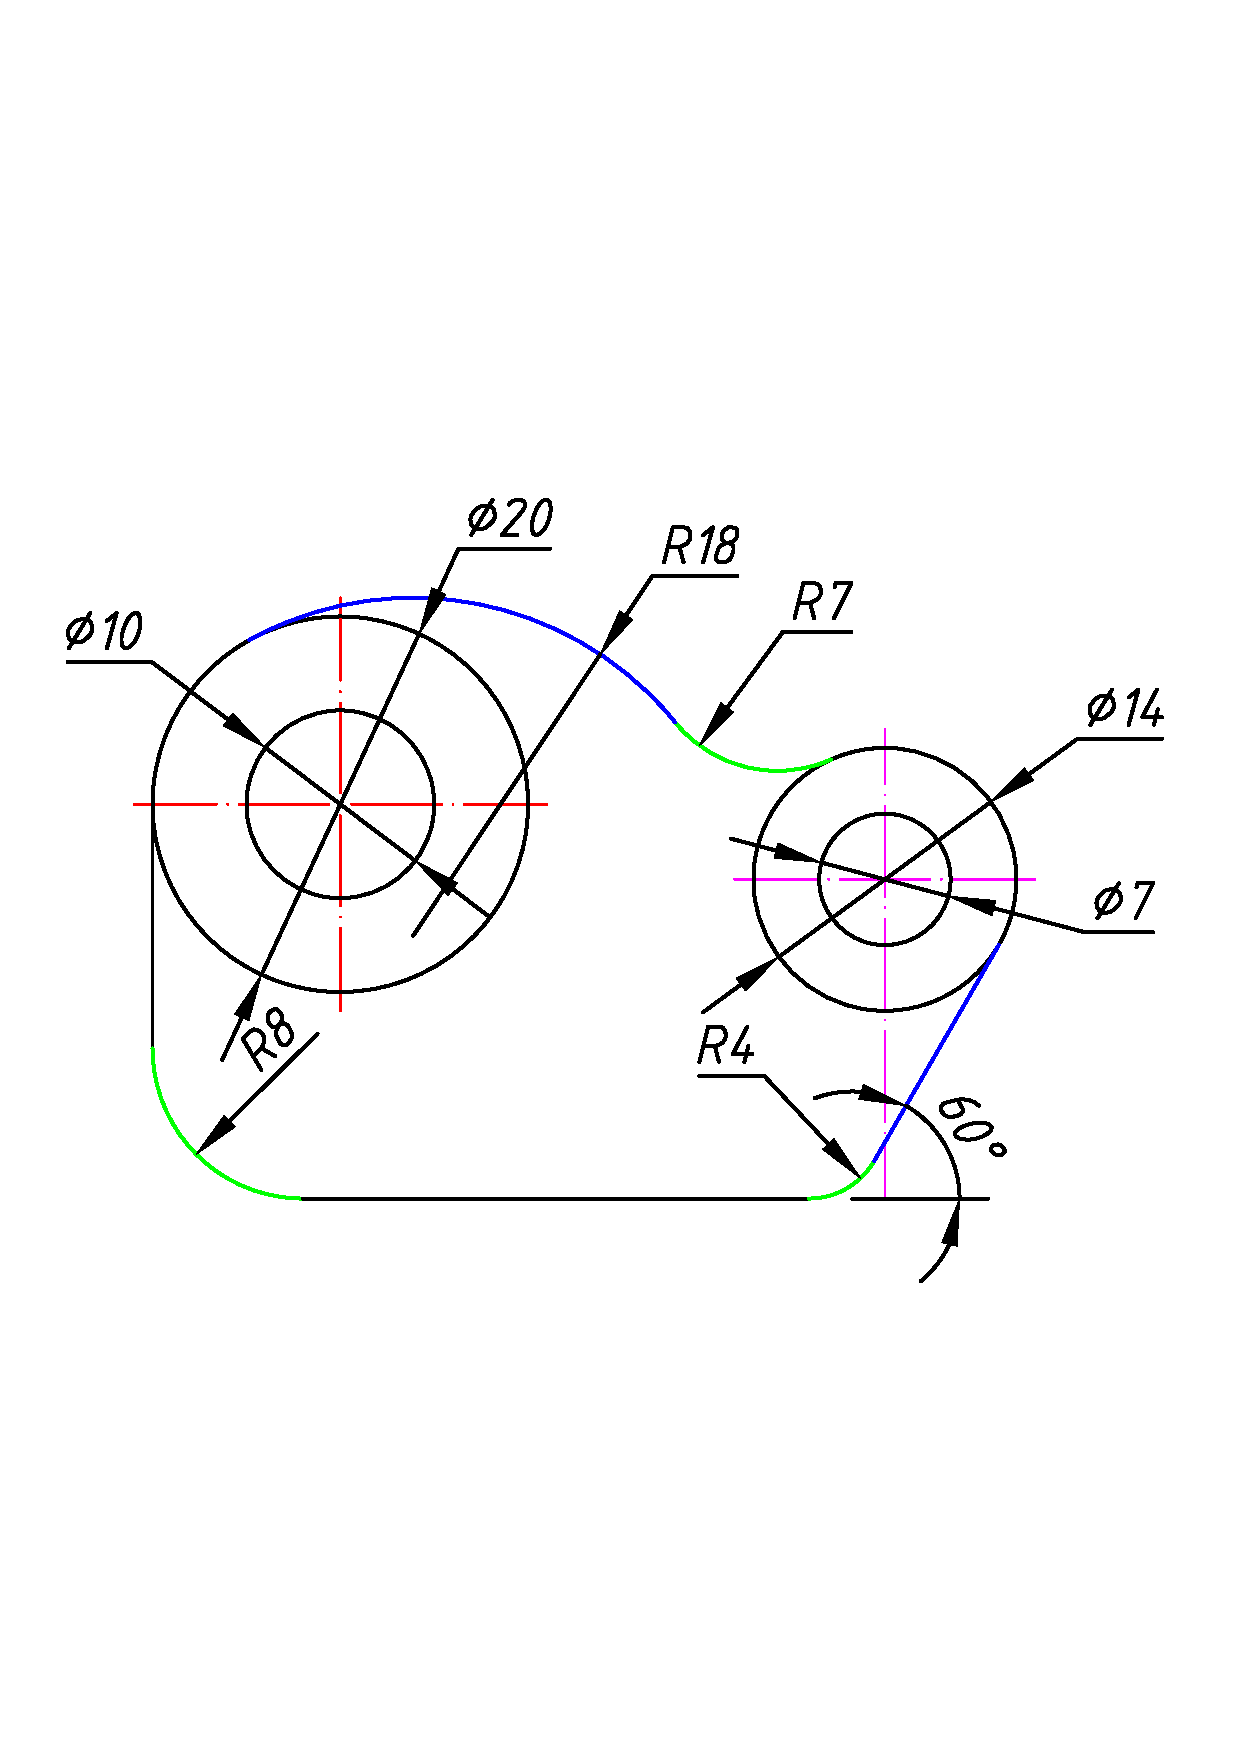
\includegraphics[scale=0.35]{biaozu6.pdf}
}
\ffigbox{\caption{定位尺寸}\label{fig:biaozu5}}{
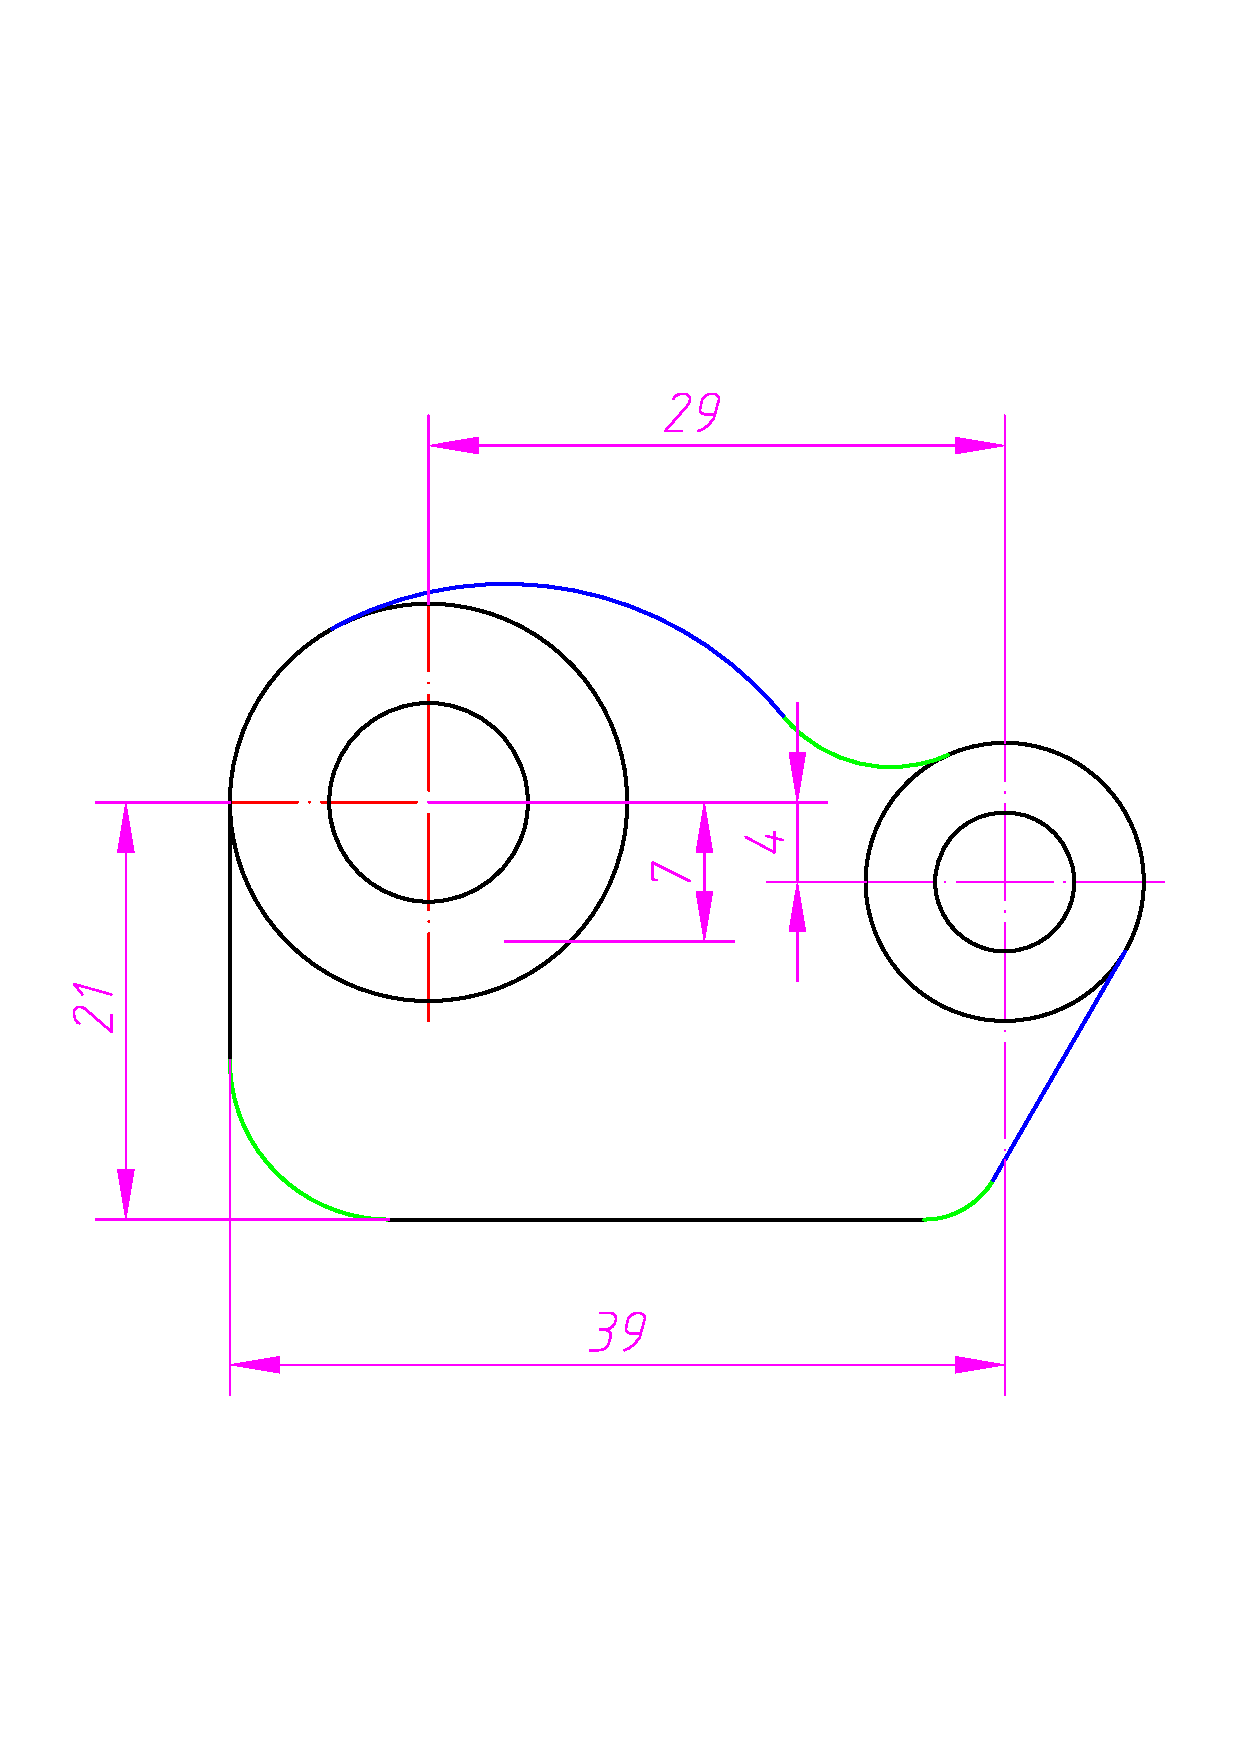
\includegraphics[scale=0.3]{biaozu5.pdf}
}
\end{floatrow}
\end{figure}
\indent

\item 定位尺寸

定位尺寸是确定平面图形中各线段之间相对位置的尺寸,如图\ref{fig:biaozu5}所标出的尺寸均为图\ref{fig:biaozu}的定位尺寸,其中4和29用于确定$\phi 14$圆的圆心位置。

\end{enumerate}
\subsection{平面图形中线段性质的分析}
平面图形中各线段(直线或圆弧)的定位尺寸的数量将直接影响绘图先后顺序,因此可将线段分为以下三类。

\begin{enumerate}
\item 已知线段

已知线段是有足够的定形尺寸,不需要利用与其它线段的连接关系即可直接画出的直线或圆弧。图\ref{fig:biaozu2}所示的即为图\ref{fig:biaozu}的已知线段。

\item 中间线段

中间线段是缺少一个定位尺寸,需要通过与它相邻某一边的图线的连接关系,才能够作出的直线或圆弧。图\ref{fig:biaozu3}在图\ref{fig:biaozu2}的基础上绘制出所有的中间线段。
\item 连接线段

连接线段是缺少两定位尺寸,需要通过与它相邻两边图形的相切关系,才能够作出的直线或圆弧。图\ref{fig:biaozu4}在图\ref{fig:biaozu3}的基础上进一步添加所有的连接线段。
\end{enumerate}

\noindent
\begin{figure}[htbp]
\centering
\subfloat[已知线段]{\label{fig:biaozu2}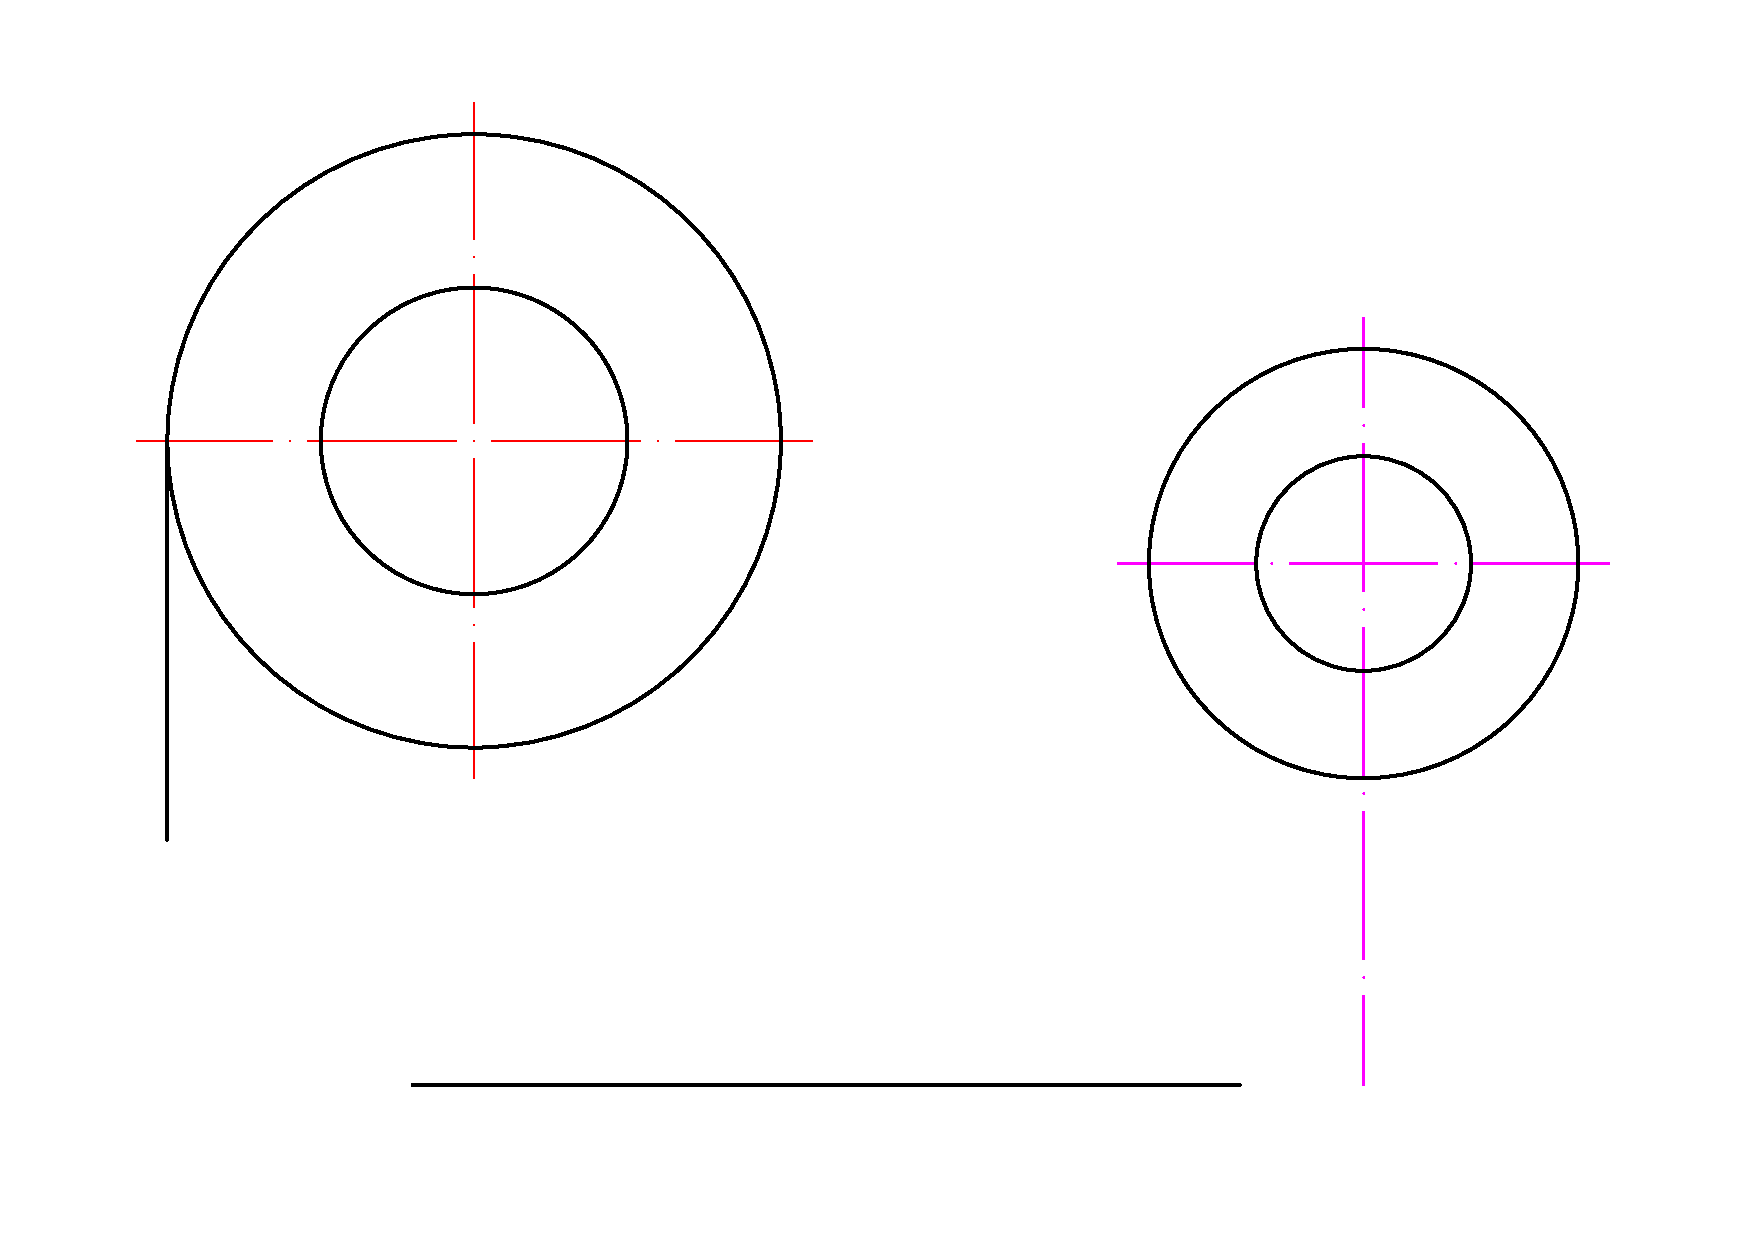
\includegraphics[scale=0.15]{biaozu2.pdf}}\hspace{20pt}
\subfloat[中间线段]{\label{fig:biaozu3}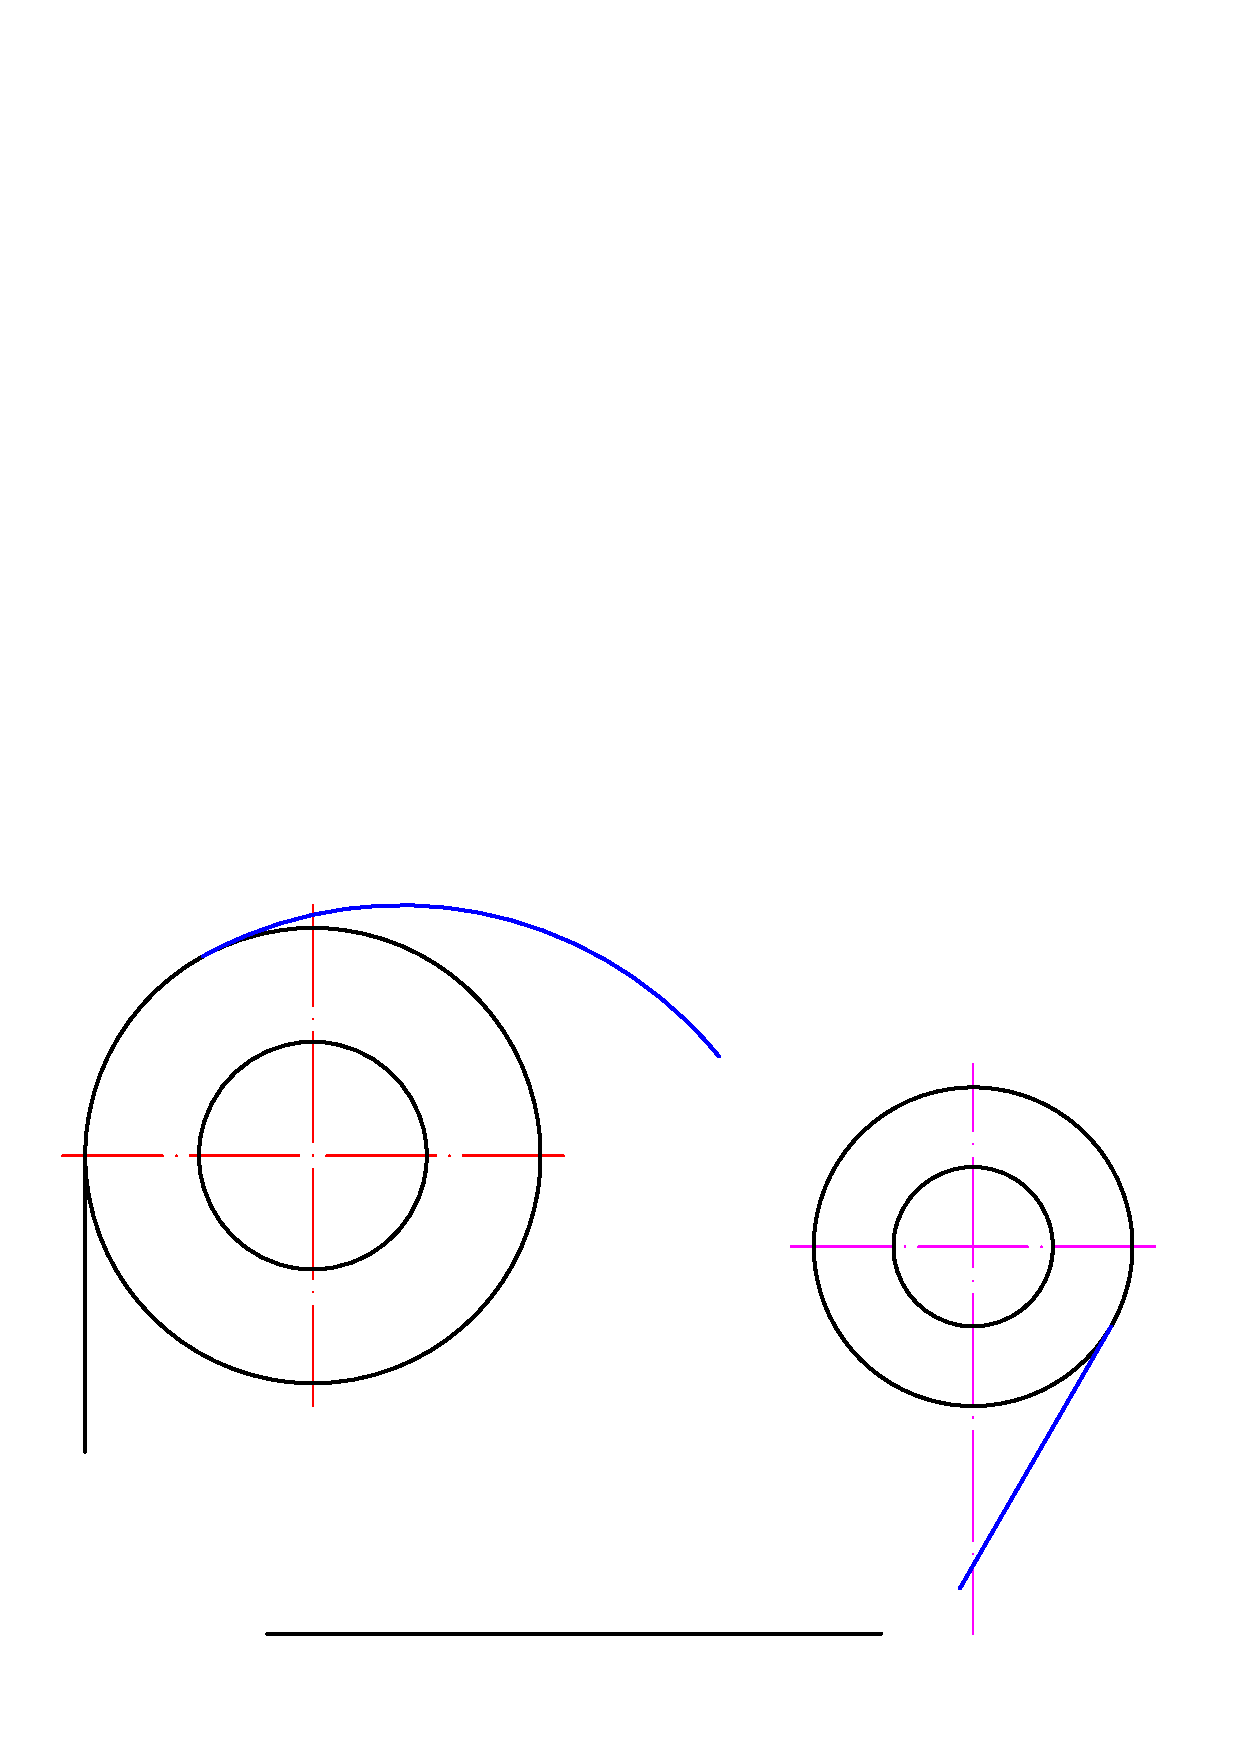
\includegraphics[scale=0.2]{biaozu3.pdf}}\hspace{20pt}
\subfloat[连接线段]{\label{fig:biaozu4}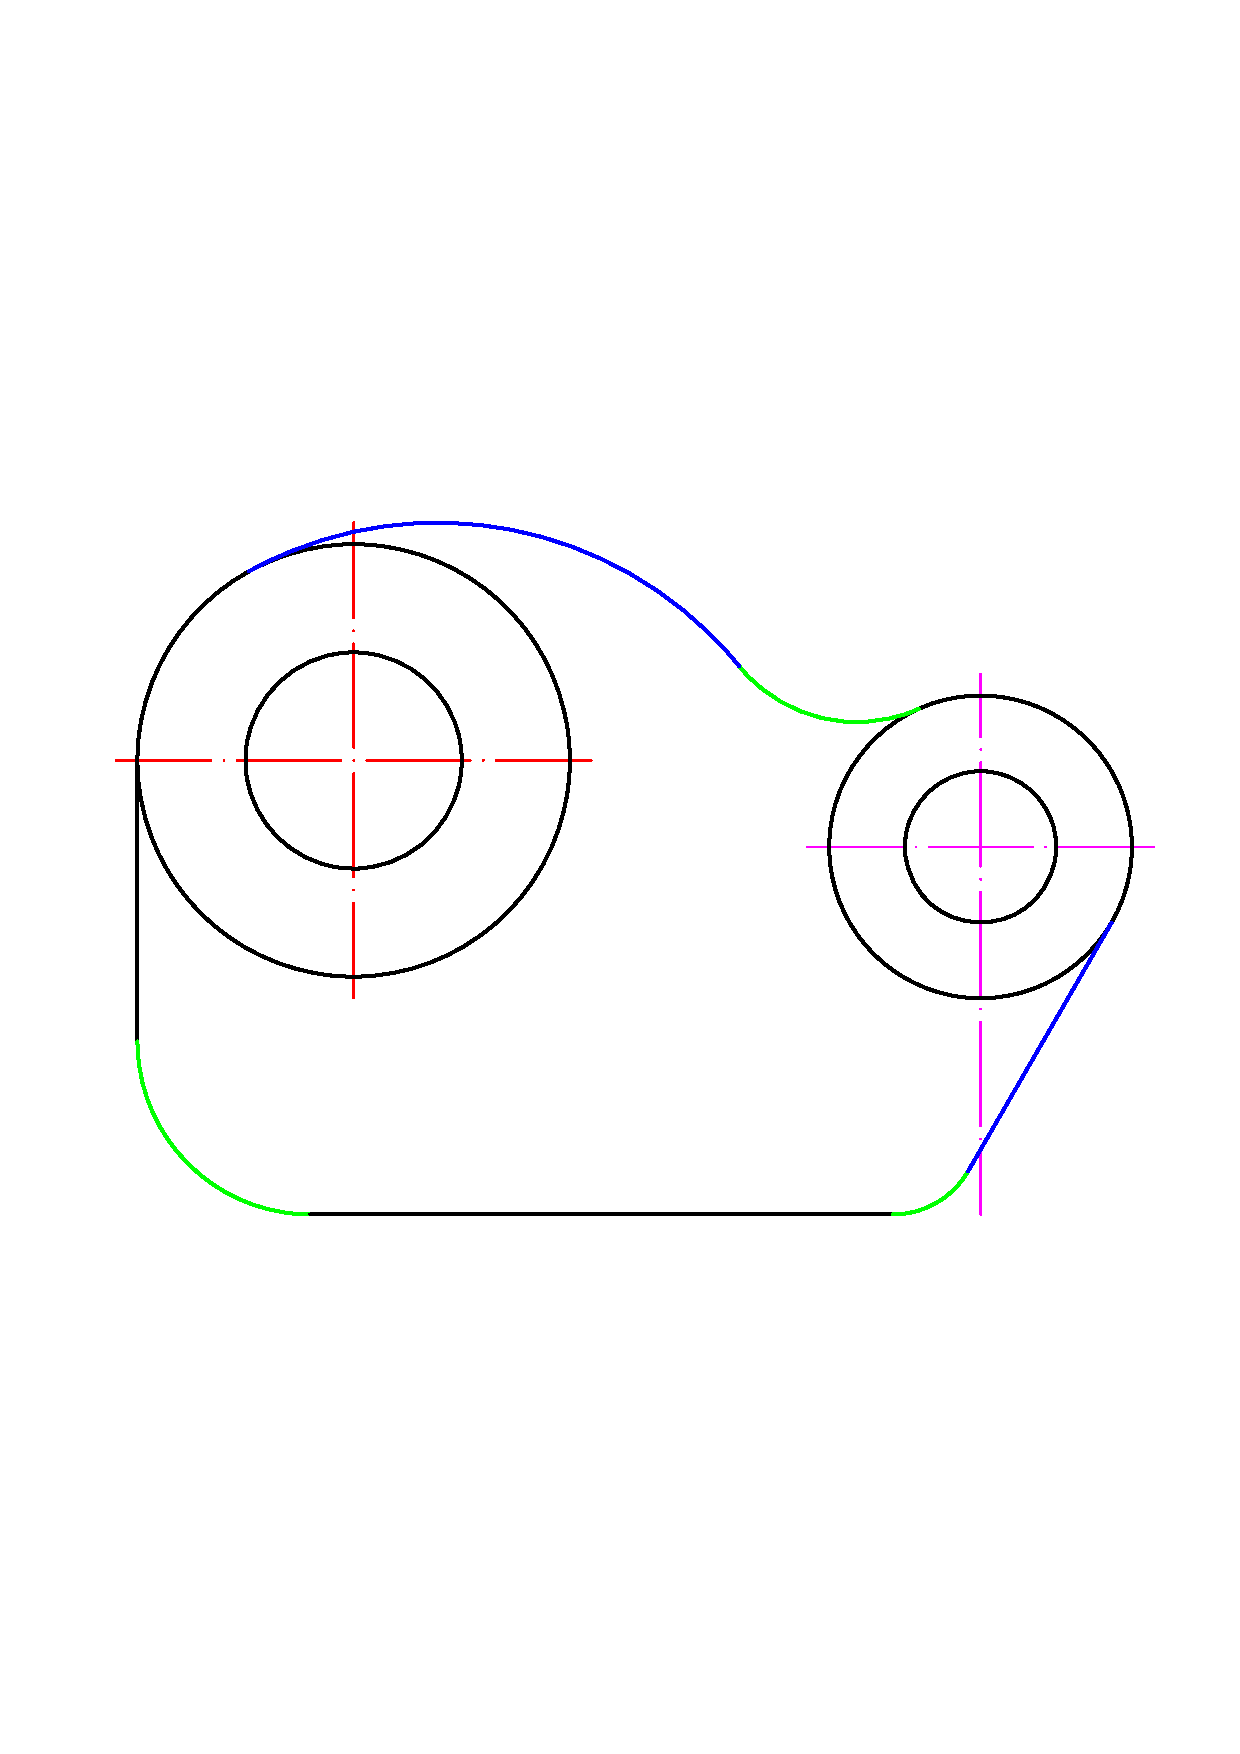
\includegraphics[scale=0.2]{biaozu4.pdf}}
\caption{平面图形中的线段分析}
\end{figure}
\indent
\clearpage
\endinput